
%%==================================================
%% demo.tex for BIT Thesis
%% modified by yang yating
%% version: 1.2
%% last update: Jan. 4th, 2018
%%==================================================

% 默认单面打印 oneside 、硕士论文模板 master

\documentclass[oneside, master]{BIT-thesis-grd}

% 模板选项: 硕士论文 master; 博士论文 doctor

%==============更改数学字体设置,Latin Modern Math 默认的的确有点细,看个人需要,下面提供一种方法,需要的可以取消注释=========%

% \usepackage[bold-style=ISO]{unicode-math} %采用unicode-math,可以直接输入Unicode公式,当然传统的输入就行
% \setmathfont{XITS Math}  %目前unicode-math 支持几种数学字体,具体用法可以查看帮助文档,这里采用类似times字体科学数学字体,可以取消注释对比


\begin{document}

%%%%%%%%%%%%%%%%%%%%%%%%%%%%%%
%% 封面
%%%%%%%%%%%%%%%%%%%%%%%%%%%%%%

% 中文封面内容(关注内容而不是表现形式)
\classification{TQ028.1}
\UDC{540}

\title{固定翼紧密编队控制及应用}
\vtitle{固定翼紧密编队控制及应用}
\author{李 顺}
\institute{宇航学院}
\advisor{王佳楠教授}
\chairman{王佳楠教授}
\degree{工学学士}
\major{飞行器设计与工程}
\school{北京理工大学}
\defenddate{2020年3月}
%\studentnumber{**********}


% 英文封面内容(关注内容而不是表现形式)
\englishtitle{Close Formation Control and Application of Fixed-wing UAV}
\englishauthor{Shun Li}
\englishadvisor{Prof. J.N. Wang}
\englishchairman{Prof. J.N. Wang}
\englishschool{Beijing Institute of Technology}
\englishinstitute{School of Aerospace Engineering}
\englishdegree{Bachelor of Engineering}
\englishmajor{Aircraft Design and Engineering}
\englishdate{03,2020}

% 封面绘制
\maketitle

% 中文信息
\makeInfo

% 英文信息
\makeEnglishInfo

%打印竖排论文题目
\makeVerticalTitle

% 论文原创性声明和使用授权
\makeDeclareOriginal

%%%%%%%%%%%%%%%%%%%%%%%%%%%%%%
%% 前置部分
%%%%%%%%%%%%%%%%%%%%%%%%%%%%%%
\frontmatter

% 摘要
%%==================================================
%% abstract.tex for BIT Master Thesis
%% modified by yang yating
%% version: 0.1
%% last update: Dec 25th, 2016
%%==================================================

\begin{abstract}
本文……。({\color{blue}{摘要是一篇具有独立性和完整性的短文,应概括而扼要地反映出本论文的主要内容。包括研究目的、研究方法、研究结果和结论等,特别要突出研究结果和结论。中文摘要力求语言精炼准确,硕士学位论文摘要建议500$\sim$800字,博士学位论文建议1000$\sim$1200字。摘要中不可出现参考文献、图、表、化学结构式、非公知公用的符号和术语。英文摘要与中文摘要的内容应一致。}})

\keywords{形状记忆; 聚氨酯; 织物; 合成; 应用 ({\color{blue}{一般选3~8个单词或专业术语,且中英文关键词必须对应。})}}
\end{abstract}

\begin{englishabstract}

   In order to exploit …….
   
\englishkeywords{shape memory properties; polyurethane; textile; synthesis; application}

\end{englishabstract}

%% 符号对照表,可选,如不用可注释掉
\begin{denotation}
	
\item[$V_g$] 无人机地速向量
\item[$V_a$] 无人机空速向量  


\end{denotation}

% 加入目录
\tableofcontents


%加入图、表索引(同时取消图表索引中章之间的垂直间隔)
\let\origaddvspace\addvspace
\renewcommand{\addvspace}[1]{}
\listoffigures
\listoftables
\renewcommand{\addvspace}[1]{\origaddvspace{#1}}



%%%%%%%%%%%%%%%%%%%%%%%%%%%%%%
%% 正主体部分
%%%%%%%%%%%%%%%%%%%%%%%%%%%%%%
\mainmatter

%% 各章正文内容
%%==================================================
%% chapter01.tex for BIT Master Thesis
%% modified by yang yating
%% version: 0.1
%% last update: Dec 25th, 2016
%%==================================================
\chapter{绪论}
\label{chap:intro}
\section{本论文研究的目的和意义}
在未来战争中,仅靠单架无人机自主作战无法适应复杂多样的战场环境,而具备协同作战的无人机编队能更好地完成任务,与单架无人机相比具有作战效率高、
视野广阔等优势,可实现对目标的全方位立体监视,对地精确攻击。另外,无人机紧密编队可以实现长航任务中无人机的空中加油,对接等任务,如图\ref{fig:c01-meaning-1}。
编队飞行作为无人机研究领域的热点与难点问题,涉及多项关键技术,例如:队形设计、自主编队、队形保持变换、协调通信等。无人机自主编队控制是实现集群作战的关键技
术。

固定翼无人机以紧密编队的形式飞行,如迁徙的鸟儿一样,可以减少整体的飞行阻力并且减少燃料消耗。整体编队产生的效果将会与精心设计的、具有良好的气动
外形的飞行器相媲美。但是,按照相关文献显示,如果固定翼编队的控制精度无法达到要求精度的10\%,那么最优的减租效果可能会被削减30\%。
\begin{figure}
  \centering
  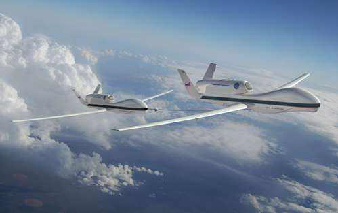
\includegraphics[width=0.5\textwidth]{figures/c01-meaning-1}
  \caption{无人机编队加受油}\label{fig:c01-meaning-1}
 \end{figure}
%\upcite{Takahashi1996Structure,Xia2002Analysis,Jiang1989,Mao2000Motion,Feng1998}%这个是文献引用上标
\section{国内外研究现状及发展趋势}
%\label{sec:***} 可标注label
现如今的无人机自动驾驶仪的结构多为导航模块、位置控制控制模块(外环)以及姿态控制模块(内环);导航模块产生期望位置,位置控制模块由期望位置产生
期望姿态角,姿态控制模块由期望姿态角产生最终的伺服系统的控制量。现如今的低成本无人机所使用的传感器硬件精度比较低,均为消费级别,如果不考虑传感
器的精度问题而设计控制方案,很可能导致整体编队的控制精度下降。现如今已经存在的大部分编队控制算法,未考虑无人机的动力学模型,即只考虑飞机的质点
运动学以及质点动力学条件下提出的导航方法,最终产生的飞行器的控制量为无人机航迹坐标系下的加速度期望值。按照飞机的控制方式,需要将航迹坐标系下的
期望控制量转到机体系之下,但是飞机自动驾驶仪并不能接受加速度控制量,尤其是飞机机体x轴方向,无人机推力、阻力以及重力沿机体方向的推力并非是代数关
系,不能直接由期望加速度得到期望推力;另外由于低成本无人机的惯性原件的精度问题导致无人机不能使用测量的加速度信息作为反馈,两种原因导致以加速度
为最终控制量对于低成本无人机编队的方法控制精度不足。

%TODO:此处的引用存疑
目前的编队控制已经提出多种方案,例如:基于距离的编队控制策略、人工势场法,基于距离的编队控制,基于行为的编队控制,基于虚拟结构的编队控制,基于虚
拟领机的编队控制等。其中,基于距离编队中的领从模式因其原理简单而得到广泛应用。本文正是给予领从策略(leader-follower method)设计的编队控制器。
\section{本文的技术方案}
%\label{sec:***} 可标注label
首先建立无人机编队的领机与从机相对运动模型,描述领机从机在三维空间之内的运动规律。其次按照编队的控制目标设计编队控制器的误差输入量,并按照无人机
的内环的输入量,设计编队控制的数学形式。之后再完成无人机质点模型下的编队控制率仿真,完善编队所设计编队控制器的结构。之后,利用ROS/Gazebo等仿真包搭建
无人机编队动力学仿真环境,测试编队控制再考虑自动驾驶仪内环以及无人机的动力学模型之后的编队控制表现。最后,进行实际飞行的测试:记录编队控制的实际动态特性
稳态特性、飞行编队的抗干扰能力、以及编队的能源节约情况。
\section{本文的组织结构}
本文之后的部分将如下组织:第二章建立无人机编队的动力学模型;第三章设计编队控制器数学形式;第四章介绍无人机编队整体控制逻辑、仿真环境以及硬件选型
;第五章控制器仿真以及实际飞行实验结果分析;第六章为结论。
\chapter{小型无人机动力学模型的建立}
\label{chap:formation_dynamic_equ}
本章基于无人机编队的领从方法(leader-follower method)建立无人机编队的相对运动方程。为了与无人机自动驾驶仪的解耦控制方法相匹配,本文将无人机
空间运动划分为水平平面运动以及竖直平面运动,并在两个平面
内分别建立数学模型。由于无人机尺寸小,强度大,飞行包线较小,现做如下假设:
\begin{itemize}
    \item 无人机为具有6运动自由度的三维空间刚体。
    \item 忽略地球自转,将地球作为惯性系处理。
    \item 忽略地球曲率,即所谓的“平板地球假设”。\cite{Wusentang2013}
    \item 由于内环控制率以无人机协调(倾斜)转弯(STT)为基础(详见第\ref{chap:hardware}章),飞机满足无侧滑条件,假定侧滑角为0;即空速方向与机体系$O_bx_b$在同一竖直平面内。
    \item 由于编队飞行时的区域较小,领机与从机的大气环境以及地球重力场等因素完全一致。
\end{itemize}
本章中涉及的坐标系有:
\begin{enumerate}
    \item 地面坐标系$O_gx_gy_gz_g$:原点$O_g$点选为无人机自动驾驶仪解锁时的位置,$O_gx_g$轴指向地理北极,$O_gy_g$轴指向东,$O_gz_g$轴符合右手定则,
        指向下。
    \item 导航坐标系$NED(north-east-down)$:原点选作无人机质心,$N$轴指向地理北极,$E$轴指向东,$D$轴符合右手定则,指向下。
    \item 航迹坐标系$O_kx_ky_kz_k$:原点$O_k$选为无人机质心,$O_kx_k$轴始终指向无人机地速矢量方向,$O_kz_k$轴位于包含$O_kx_k$轴的竖直平面内,
        $o_ky_k$符合右手定则,指向右。
    \item 机体坐标系$O_bx_by_bz_b$:原点$O_b$选为无人机质心,$O_bx_b$位于无人机的对称平面内,平行于机身轴线或者机翼的平均气动弦线,指向无人机机身前方;
        $O_bz_b$亦在对称平面之内,垂直于$O_bx_b$轴,指向下;$O_by_b$垂直于对称平面,指向右。多数情况下,无人机操纵机构产生的力矩在该坐标系中定义。
    \item 气流坐标系$O_ax_ay_az_a$:气流坐标系又被称作风坐标系或者速度坐标系;原点$O_a$取作无人机质心,$O_ax_a$始终指向无人机的来流方向的相反方向,
        即空速矢量方向;$O_az_a$位于无人机对称面之内,
        垂直于$O_ax_a$轴,指向下;$O_ay_a$轴符合右手定则,垂直于$O_ax_az_a$平面,指向右。只有在大气风速$V_{wind}=0$时,航迹系的$O_kx_k$才与气流坐标系的
        $O_ax_a$重合。
\end{enumerate}
本章中领机与从机的各运动学量以及几何关系分别用上标$l,f$标记,从机期望值以$“des”$上标标记;
运动学量以及几何关系所属坐标系关系则用各个坐标系的字母作为下标标记。
领机、从机在水平以及竖直平面内的几何关系分别在图\ref{fig:c02-2d_level_motion}和图\ref{fig:c02-2d_vert_motion}给出;
\begin{figure}[H]
    \centering
    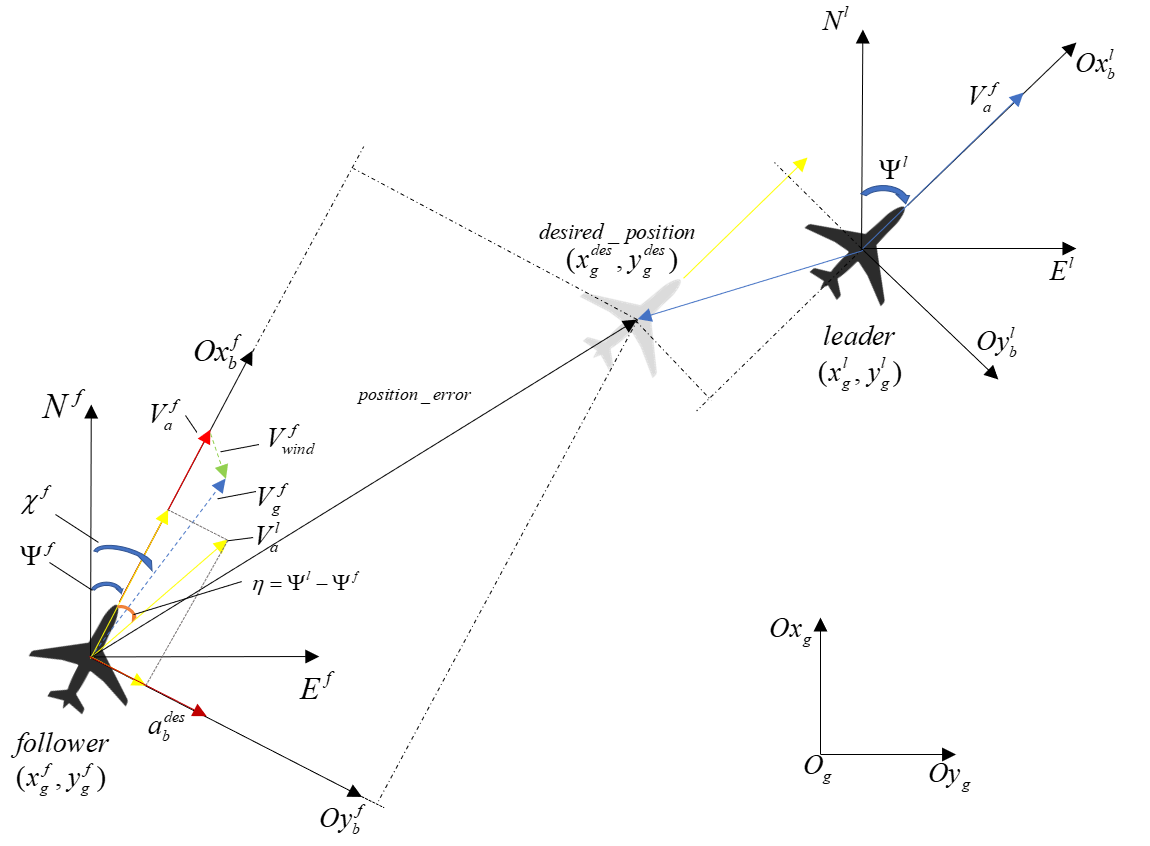
\includegraphics[width=0.75\textwidth]{figures/c2/2d_level_motion.png}
    \caption{水平平面双机编队几何关系}\label{fig:c02-2d_level_motion}
\end{figure}
\begin{figure}[H]
    \centering
    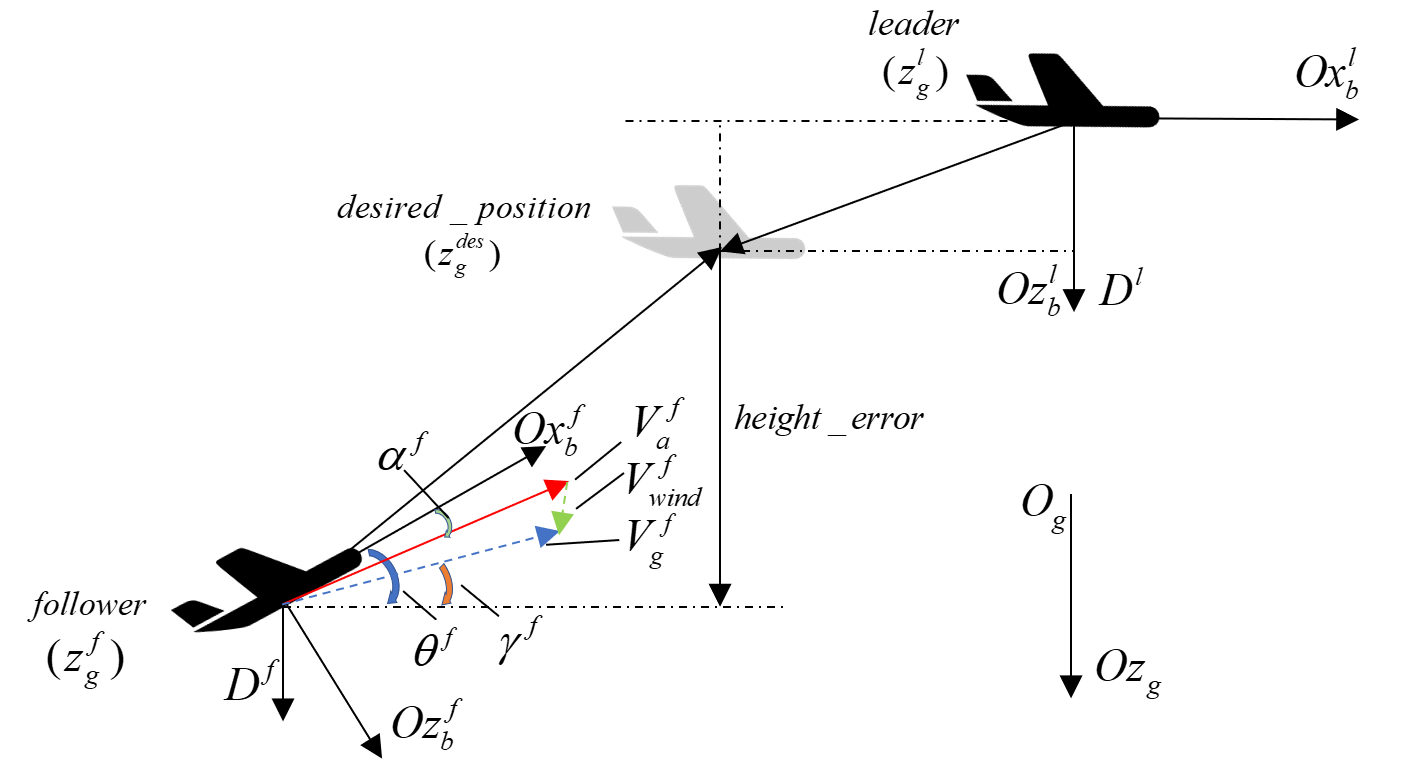
\includegraphics[width=0.75\textwidth]{figures/c2/2d_vert_motion.png}
    \caption{竖直平面双机编队几何关系}\label{fig:c02-2d_vert_motion}
\end{figure}
在图\ref{fig:c02-2d_level_motion}中:
$(x_{g}^l,y_{g}^l),(x_{g}^f,y_{g}^f),(x_{g}^{des},y_{g}^{des})$分别为领机、从机以及从机期望编队位置在地面坐标系$O_gx_gy_g$平面之中的分量;
$\Psi^l,\Psi^f$分别为领机与从机的偏航角(yaw angle);
$\chi^l,\chi^f$分别为领机与从机的航迹偏角(航迹方位角);
$V_a,V_{wind},V_g$分别为领机和从机的空速、风速以及地速向量;
$a_{b}^{des}$是从机产生的、在体轴系下的期望的法向加速度。

在图\ref{fig:c02-2d_vert_motion}中:
$z_{g}^l,,z_{g}^f,z_{g}^{des}$分别为领机、从机以及从机期望编队位置在地面坐标系$O_gz_g$轴上的分量;
$\theta^l,\theta^f$分别为领机与从机的俯仰角(pitch angle);
$\gamma^l,\gamma^f$分别为领机与从机的航迹倾角(航迹倾斜角);
$V_a,V_{wind},V_g$分别为领机和从机的空速、风速以及地速向量;

在图\ref{fig:c02-2d_level_motion}和图\ref{fig:c02-2d_vert_motion}中,由飞机飞行动力学可知,从机与领机三维运动学方程均为:
\begin{equation}
    \left\{
    \begin{array}{l}
        \frac{dx_g}{dt}=V_g\cos\gamma\cos\chi\\
        \frac{dy_g}{dt}=V_g\cos\gamma\sin\chi\\
        \frac{dz_g}{dt}=-V_g\sin\gamma
    \end{array}
    \right .
    \label{fol_motion_eauation}
\end{equation}
现考虑无风情况下,则由图\ref{fig:c02-2d_level_motion}可知,无人机航迹偏角等于航向角,即$\Psi=\chi$;无人机在平衡状态下,迎角很小(本无人机约在2.3°左右),由图\ref{fig:c02-2d_vert_motion}可得$\theta\approx\gamma$。
于是方程组\ref{fol_motion_eauation}可改写为:
\begin{equation}
    \left\{
    \begin{array}{l}
        \frac{dx_g}{dt}=V_g\cos\theta\cos\Psi\\
        \frac{dy_g}{dt}=V_g\cos\theta\sin\Psi\\
        \frac{dz_g}{dt}=-V_g\sin\theta
    \end{array}
    \right .
    \label{fol_motion_eauation1}
\end{equation}
方程组\ref{fol_motion_eauation1}的第1、2两式表示无人机在水平平面内的运动轨迹;第3式表示无人机在竖直平面内的运动轨迹。方程组中,控制的直接输入量为从机的$V_{g}^f,\theta^f,\Psi^f$,再确定飞机的初始运动量之后,可唯一确定领机与从机的
运动规律。

值得注意的是:上述控制量并不能直接由编队控制器产生,但经过理想内环控制器以及无人机动力学模型之后,将产生相应的上述的直接控制量,完整流程将在第\ref{chap:controller_design}章中介绍。

\chapter{编队控制器设计}
\label{chap:controller_design}
第\ref{chap:formation_dynamic_equ}章中介绍了无人机双机编队的动力学模型,并将无人机运动分为铅垂平面以及水平平面;方程组\ref{fol_motion_eauation1}水平平面的直接输入量为$\Psi$的期望值,铅垂平面的
直接输入量为$\theta$和$V$的期望值。整体的控制逻辑框图如下图所示:
\begin{figure}[H]
    \centering
    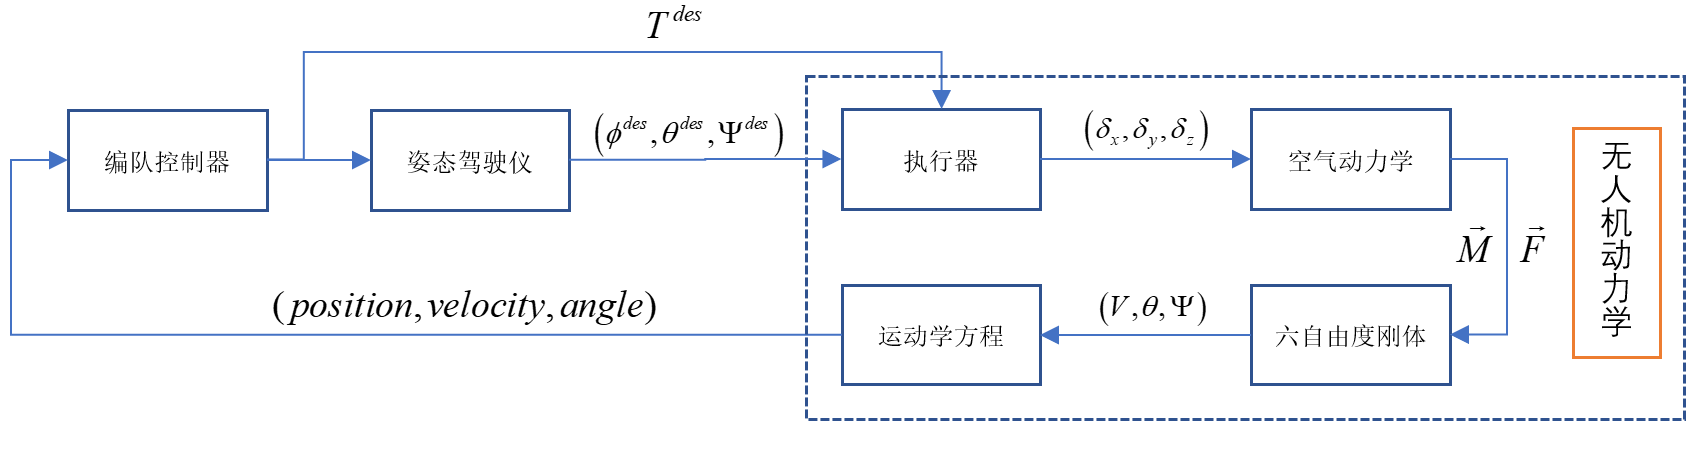
\includegraphics[width=0.85\textwidth]{figures/c3/c3-overview_controller.png}
    \caption{控制逻辑框图}\label{fig:c3-overview_controller}
\end{figure}
编队控制器的输入为定义的误差量,输出为无人机自动驾驶仪的内环输入值,即期望推力$T^{des}$,期望姿态$\Phi^{des},\theta^{des}$,偏航期望值$\Psi^{des}$将由内环姿态
自动驾驶仪按照协调转弯条件计算得到。本章的剩余部分将分别设计铅垂平面以及水平平面的控制器。

需要说明的是:本章前两节先假设大气静止,设计无风条件下的编队控制器,第三节再引入风的干扰,并做相应处理。根据第二章的坐标系的定义,此假设将使得航迹坐标系与速度坐标系重合,又因为“无侧滑条件”(也称作协调转弯条件,BTT)的引入,机体二维水平平面坐标系$O_bx_by_b$将与前二者的水平平面坐标系($O_kx_ky_k$和$O_ax_ay_a$)重合。进而控制器产生的控制量与执行机构恰好对应,因此前两节之中,上述三种二维平面坐标系将不做区分。下面将选取航迹坐标系设计编队控制器。
\section{水平平面编队控制器设计}
\subsection{误差定义}
导航与制导的本质是控制地速的方向,实现手段是产生垂直于速度方向的法向加速度$a_{y_k}^{des}$;因而本章中误差以及控制量全部定义在航迹坐标系$O_kx_ky_kz_k$之中。但编队控制器不仅要控制速度的方向,还要控制速度的大小,以实现与领机的同步飞行。编队控制的最终目标为:
\begin{enumerate}
    \item 从机速度方向与领机的速度方向一致。
    \item 从机的速度大小与领机的速度大小一致。
    \item 从机的位置与从机的期望位置一致。
\end{enumerate}
此处产生三种误差类型,这三类误差均投影在从机航迹坐标系$O_kx_ky_kz_k$之中,便于之后对应要控制的物理量产生控制量:
\begin{enumerate}
    \item 领机与从机2维速度方向误差$\eta$,参见图\ref{fig:c02-2d_level_motion}。%TODO:记得改一下图,与之对应
    \item 领机与从机速度(地速$V_g$)大小误差$|V_g|^{err}$。
    \item 领机与从机3维位置误差$(P_{x_k}^{err},P_{y_k}^{err},P_{z_k}^{err})$
\end{enumerate}
因而此处水平平面的编队控制器的控制的任务是消除水平平面内的位置误差、速度大小以及速度方向误差,前两者在$O_kx_k$轴的分量需通过期望速度大小${|V|}_{x_k}^{des}$消除;前两者在$O_ky_k$轴
的分量,以及速度方向误差须通过期望法向加速度$a_{y_k}^{des}$消除。值得注意的是:实际上此处的速度方向误差代表了航迹系内的两分量之比值,实际上与角度误差代表同一误差,但是由于航迹系$O_kx_k$轴
的期望速度时刻变化,而所需的速度方向须按照领机速度方向一致,因而要控制速度的方向,而不是单纯的$O_kx_k$轴的速度分量。
\subsection{航迹系x轴方向控制器}
航迹系$O_kx_k$轴方向的控制器的输入为速度大小误差以及位置误差沿本轴分量的混合,控制器选用增量式离散$PID$控制器,最终的控制量的输出为航迹坐标系$O_kx_k$轴期望速度大小${|V|}_{x_k}^{des}$。控制器的表达式为:
\begin{equation}
    \left\{
    \begin{array}{l}
        |V_g|^{err}(k)=|V_g^{l}|(k)-|V_g^{f}|(k)\\
        P_{x_k}^{err}(k)=P_{x_g}^{des}(k)-P_{x_g}^{f}(k)\\
        e_{x_k}(k)=K_V|V_g|^{err}(k)+K_{Px}P_{x_k}^{err}(k)\\
        \begin{aligned}
        \Delta{|V|}_{x_k}^{des}(k)=&K_{p}^{xmix}[e_{x_k}(k)-e_{x_k}(k-1)]+K_{i}^{xmix}e_{x_k}(k)+\\
        &K_{d}^{xmix}[e_{x_k}(k)-2e_{x_k}(k-1)+e_{x_k}(k-2)]
        \end{aligned}
        \\
        {|V|}_{x_k}^{des}(k)=\Delta{|V|}_{x_k}^{des}(k)+{|V|}_{x_k}^{des}(k-1)
    \end{array}
    \right .
    \label{xk_vel_gen_equ}
\end{equation}
其中,前3式定义了混合误差形式,实际为速度误差与位置误差的线性叠加。后2式表示了最终的期望速度大小的产生。$k$为控制器第$k$次采样计算;$K_V,K_P$为误差线性混合常;$K_{p}^{xmix},K_{i}^{xmix},K_{d}^{xmix}$为增量式离散
$PID$控制器参数。

此处产生的期望速度大小,并不能直接为内环姿态驾驶仪所响应,需要经过铅垂平面控制器的计算,位置误差$P_{z_k}^{err}$共同产生期望油门以及期望俯仰角。
\subsection{航迹系y轴方向控制器}
航迹系$O_ky_k$轴方向的控制器的输入为速度方向误差$\eta$以及位置误差的混合,类似于航迹系$O_kx_k$轴方向的控制器,控制器也选用增量式离散$PID$控制器,最终的输出为无人机滚转角期望值。
由图\ref{fig:c02-2d_level_motion}可得到:
\begin{equation}
    \eta^f=\Psi^l-\Psi^f
    \label{yaw_error}
\end{equation}
上式得到的是无人机速度方向的角度误差;

再考虑如图所示的无人机二维平面转弯运动:
\begin{figure}[H]
    \centering
    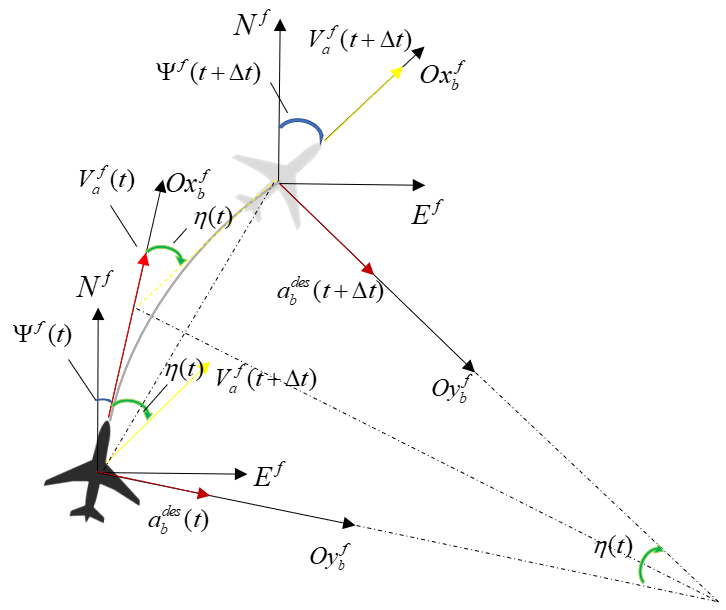
\includegraphics[width=0.5\textwidth]{figures/c3/c3-BTT.png}
    \caption{无人机二维平面转弯运动}\label{fig:c3-BTT}
\end{figure}
由于飞机速度的动力学惯性很大,在微分时间$\Delta t$时间内,速度的变化量可以忽略不计;在此时间内的偏航角增量为$\Delta\eta$,按照图中的几何关系,不难得到:
\begin{equation}
    a_{y_k}=V_g\dot{\eta}
    \label{btt_dot}
\end{equation}
上式即无人机期望偏航角速度与期望法向加速度关系。类似于上一节,定义混合误差为角度误差以及距离误差的线型混合。
再利用上一小节提出的增量式离散$PID$控制器,再综合式\ref{yaw_error},可得混合误差到期望法向加速度的表达式为:
\begin{equation}
    \left\{
        \begin{array}{l}
            \eta^f(k)=\Psi^l(k)-\Psi^f(k)\\
            P_{y_k}^{err}(k)=P_{y_g}^{des}(k)-P_{y_g}^{f}(k)\\
            e_{y_k}(k)=K_{\eta}\eta^f(k)+K_{Py}P_{y_k}^{err}(k)\\
                \begin{aligned}
                \Delta\dot{\Psi}^{des}(k)=&K_{p}^{ymix}[e_{y_k}(k)-e_{y_k}(k-1)]+K_{i}^{ymix}e_{y_k}(k)+\\
                &K_{d}^{ymix}[e_{y_k}(k)-2e_{y_k}(k-1)+e_{y_k}(k-2)]
                \end{aligned}\\
            \dot{\Psi}^{des}(k)=\Delta\dot{\Psi}^{des}(k)+\dot{\Psi}^{des}(k-1)\\
            \dot{\eta}^{des}(k)=-\dot{\Psi}^{des}(k)\\
            a_{y_k}^{des}(k)=-V_g^{f}(k)\dot{\eta}^{des}(k)
    \end{array}
\right .
    \label{angle_controller}
\end{equation}
上式得到的是期望法向加速度,再利用协调转弯(BTT)条件,将期望法向加速度,转化为期望滚转角:
\begin{equation}
    \tan\Phi^{des}(k)=\frac{a_{y_k}^{des}(k)}{g}
    \label{btt_a2roll}
\end{equation}
其中,$g$为当地重力加速度常量。至此,水平平面面内可计算得到无人机的期望滚转角$\Phi^{des}$以及期望速度大小$|V|_{x_k}^{des}$
\section{铅垂平面编队控制器设计}
铅垂平面编队控制器的输入为期望速度大小$|V|_{x_k}^{des}$以及期望高度(实际代表了高度误差$P_{z_b}^{err}$),输出为期望俯仰角$\theta^{des}$以及期望推力$T^{des}$。控制器选用基于能量的总能量控制法
(total energy control system,$TECS$)。固定翼无人机的速度控制和高度控制是耦合的,即单独控制高度或速度时,另一个未被控制量将会发生变化:
下面通过飞机飞行动力学纵向运动方程简单说明:
\\方程组\ref{fol_motion_eauation1}的第三式说明:飞机高度方向的变化率与地速大以及俯仰角大小有关,且为正相关。
飞机纵向运动质心运动的动力学方程抄录如下:
\begin{equation}
    \left\{
    \begin{aligned}
    &m \frac{\mathrm{d} V}{\mathrm{d} t}=T \cos (\alpha+\varphi) \cos \beta-D-m g \sin \gamma\\
    &m V \cos \gamma \frac{\mathrm{d} \chi}{\mathrm{d} t}=T[\sin (\alpha+\varphi) \sin \mu-\cos (\alpha+\varphi) \sin \beta \cos \mu]+C \cos \mu+L \sin \mu\\
    &-m V \frac{\mathrm{d} \gamma}{\mathrm{d} t}=T[-\sin (\alpha+\varphi) \cos \mu-\cos (\alpha+\varphi) \sin \beta \sin \mu]+\operatorname{Csin} \mu-L \cos \mu+m g \cos \gamma
    \end{aligned}
    \right .
    \label{point_dynamaic}
\end{equation}
其中,$\alpha,\mu,\phi$分别为迎角,速度滚转角以及发动机安装角。
根据之前的假设,可以将第一式近似作:
\begin{equation}
    m \frac{\mathrm{d} V}{\mathrm{d} t}=T-D-m g \sin \theta
    \label{1st_point_dynamaic}
\end{equation}
因而,综合\ref{1st_point_dynamaic}、\ref{fol_motion_eauation1}两式,可以得到如下关于速度以及高度通道的控制逻辑图:
\begin{figure}[H]
    \centering
    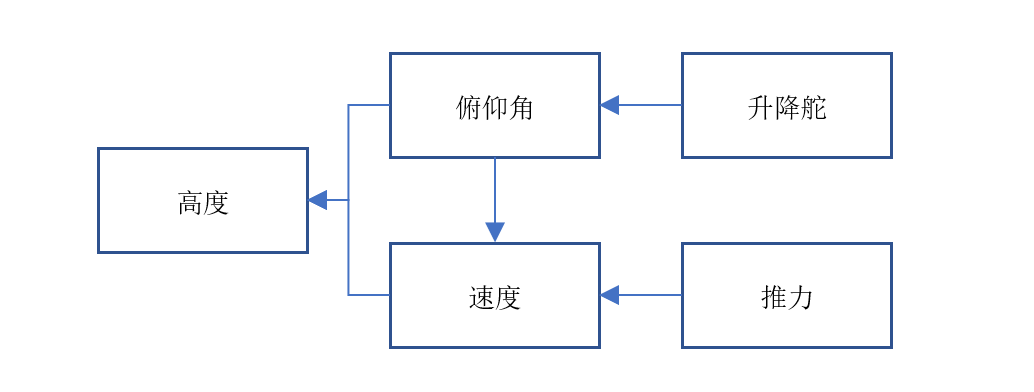
\includegraphics[width=0.75\textwidth]{figures/c3/relation_theta_thrust}
    \caption{速度以及高度通道的控制逻辑图}\label{fig:relation_theta_thrust}
\end{figure}
因而速度和高度需要同时考虑,相应的,期望俯仰角以及推力也需要同时计算。$TECS$控制器正是为此种情况设计的:%TODO:需要添加引用
所谓总能量控制(total energy control)是将无人机的速度以及高度计算得到相应的动能以及势能作为直接控制对象,应用PID控制器对动能与势能的和(total energy)
以及动能与势能的转化(total energy balance)进行控制,计算得到无人机期望俯仰角以及期望推力的控制器。飞机作为一个动力学系统,其机械能来自推力做功的输入,因而总能量控制对应着期望推力;与之对应的俯仰角控制是能量守恒的,
可作为动能向势能(反之亦然)的转化途径,对此种能量转化的控制对应着期望俯仰角。下面简要介绍$TECS$控制器的计算过程:
\\
无人机的总能量为:
\begin{equation}
    E_T=\frac{1}{2}mV_T^2+mgh
    \label{ET}
\end{equation}
对上式两边微分,可得到总能量变化率:
\begin{equation}
    \dot{E_T}=mV_T\dot{V_T}+mg\dot{h}
    \label{ET_rate}
\end{equation}
由此可得单位总能量变化率:
\begin{equation}
    \dot{E}=\frac{\dot{E}_{T}}{m g V_{T}}=\frac{\dot{V}_{T}}{g}+\frac{\dot{h}}{V_{T}}=\frac{\dot{V}_{T}}{g}+\sin \gamma
    \label{specif_ET_rate}
\end{equation}
更换式\ref{point_dynamaic}第一式形式,可得到:
\begin{equation}
    T-D=m g\left(\frac{\dot{V}_{T}}{g}+\sin \gamma\right)
    \label{point_dynamaic_change}
\end{equation}
由此可得:
\begin{equation}
    \Delta T=m g\left(\frac{\dot{V}_{T}}{g}+sin\gamma\right)
    \label{thrust}
\end{equation}
关于能量转化,定义:
\begin{equation}
    B=m g h-\frac{1}{2} m V_{T}^{2}
\end{equation}
能量转化率为:
\begin{equation}
\dot{B}=sin\gamma-\frac{\dot{V}_{T}}{g}
\end{equation}
这里参照开源软件$PX4$内部的TECS控制器设计方法,总能量环和能量分配环的控制逻辑框图如下所示:
\begin{figure}[H]
    \centering
    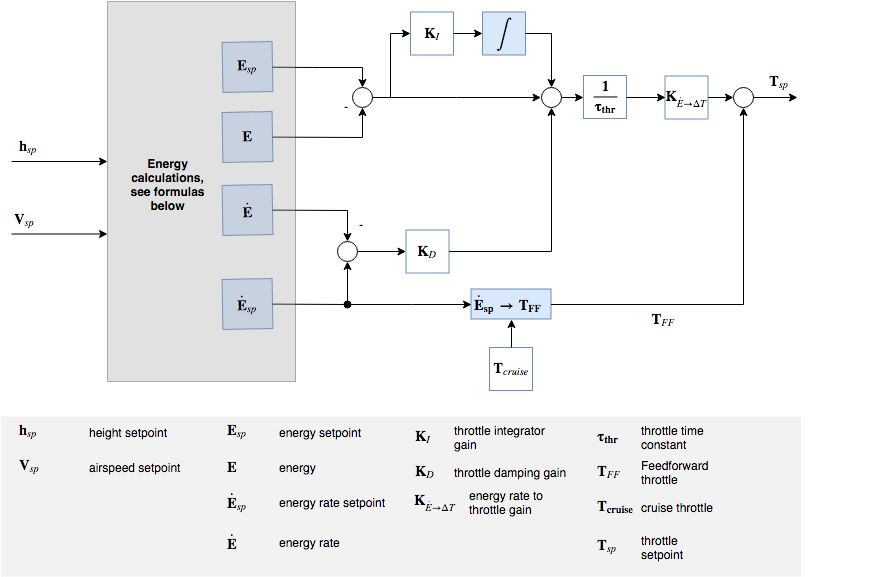
\includegraphics[width=0.75\textwidth]{figures/c3/TECS_throttle.jpg}
    \caption{总能量环}\label{fig:total_energy}
\end{figure}
\begin{figure}[H]
    \centering
    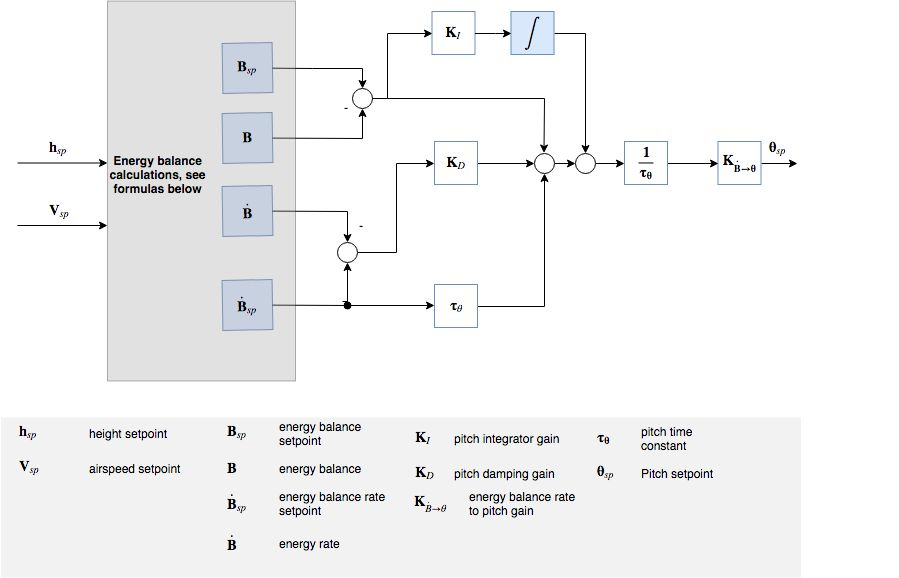
\includegraphics[width=0.75\textwidth]{figures/c3/TECS_pitch.jpg}
    \caption{能量分配环}\label{fig:balance_energy}
\end{figure}
至此,来自水平平面的期望速度$|V|_{x_k}^{des}$以及纵向平面的位置误差$P_{z_k}^{err}$将转化为期望俯仰角以及期望推力进入内环姿态驾驶仪;水平平面编队控制器
产生的期望滚转角也将进入姿态驾驶仪内环。内环姿态自动驾驶仪首先按照无侧滑条件得出期望偏航角速度$\dot{\Phi}^{des}$,然后再利用串级PID分角速度环,角
加速度环计算得到期望的执行机构的偏转角度。但现在的编队控制器还不足以直接用来进行编队控制实现,还需要经过一定的工程处理,详见下一节。
\section{实际应用时的考虑}
在实际应用编队控制器时,按照已有的经验,应主要考虑以下几个方面:
\begin{enumerate}
    \item 在无人机距离期望位置较远以及相对较近时,控制的目的是不完全一致的;应根据不同的控制需求分段设计控制律。
    \item 无人机的空速与地速差距较大(风速很大)时,地速与空速方向不能简单认为一致,应分析之后做相应的处理。
    \item 考虑到无人机各个动力学量的范围,应按照前期对于飞行平台飞行性能计算的结果对控制器计算过程中的各个物理量进行实际限幅。
    \item 离散控制器的频率问题,即内环外环频率关系应当匹配。
    \item 无人机原始信息两量测噪声问题,应设计便于使用的滤波器加以滤波。
\end{enumerate}
相应的,按照上面的问题考虑,有以下解决方案:

\subsection{编队控制器分段设计} 
在位置误差较大时,编队控制器的主要目的应为:以最大速度飞行,迅速减小距离误差;此时无人机速度的期望方向应时刻指向期望点而并非领机的速度方向。选择水平距离误差大小作为分段控制器的分段依据,定义水平距离误差为$|P|_{2d}^{err}(k)=\sqrt{[P_{x_k}^{err}(k)]^2+[P_{y_k}^{err}(k)]^2}$,决断距离记作$|P_0|_{2d}^{err}$。于是可以得到以下期望速度的表达式:
\begin{equation}
    |V|_{x_k}^{des}(k)=
    \begin{cases}
        V_{max}^f& |P|_{2d}^{err}(k)>|P_0|_{2d}^{err}\\
        \Delta{|V|}_{x_k}^{des}(k)+{|V|}_{x_k}^{des}(k-1)& |P|_{2d}^{err}(k)\leq|P_0|_{2d}^{err}
    \end{cases}
    \end{equation}
第二阶段的期望速度速度产生详见式\ref{xk_vel_gen_equ}。
关于此阶段的法向加速度的产生,此处使用××等人提出的L1控制器,将L1距离选为从机当前位置与期望位置的距离误差。其表达式如下:
\begin{equation}
    a_{y_k}^{des}(k)=
    \begin{cases}
        2\frac{V^2}{L_1}\sin{\frac{\eta}{2}}& |P|_{2d}^{err}(k)>|P_0|_{2d}^{err}\\
        -V_g^{f}(k)\dot{\eta}^{des}(k)& |P|_{2d}^{err}(k)\leq|P_0|_{2d}^{err}
    \end{cases}
    \end{equation}
上式中各运动学量参见图\ref{fig:c3-BTT},第二阶段法向加速度的产生详见式\ref{angle_controller}。再配合固定翼无人机协调转弯条件(式\ref{btt_a2roll}),可得到分段之后的期望滚转角。
\subsection{风速较大时的处理} 
\subsubsection*{风速因素对于编队控制器的影响分析}
无论导航与制导还是编队的期望速度均是对无人机的地速而言的。当内环姿态驾驶仪以无侧滑条件为基础时,若控制效果较好,则可保证侧滑角$\beta\approx 0$,即:无人机在水平二维平面运动时,空速方向与机身纵轴在同一铅垂平面内。因而飞机在平飞时,空速方向几乎与机身纵轴重合。无论有风还是无风,均有上述结论。

参照图\ref{fig:c02-2d_level_motion},当风速$V_{wind}^f$较小时,空速与地速几乎重合,且等大,此时直接将空速方向认为与空速方向一致,进而与机体方向一致的做法是可行的:前文提出的位置、角度以及速度误差均投影在航迹系$O_kx_ky_kz_b$中,所产生的修正信号$|V|_{x_k}^{des}(k),a_{y_k}^{des}(k)$与体轴系的$O_bx_b$以及$O_by_b$几乎重合,i控制机构(油门,副翼)直接相应控制信号即可,符合前文的设计。

但当风速较大时(例如,风速大小已经超过了地速的$\frac{1}{3}$,且与飞机地速有一定的角度),则会出现如下图所示的情况:
\begin{figure}[H]
    \centering
    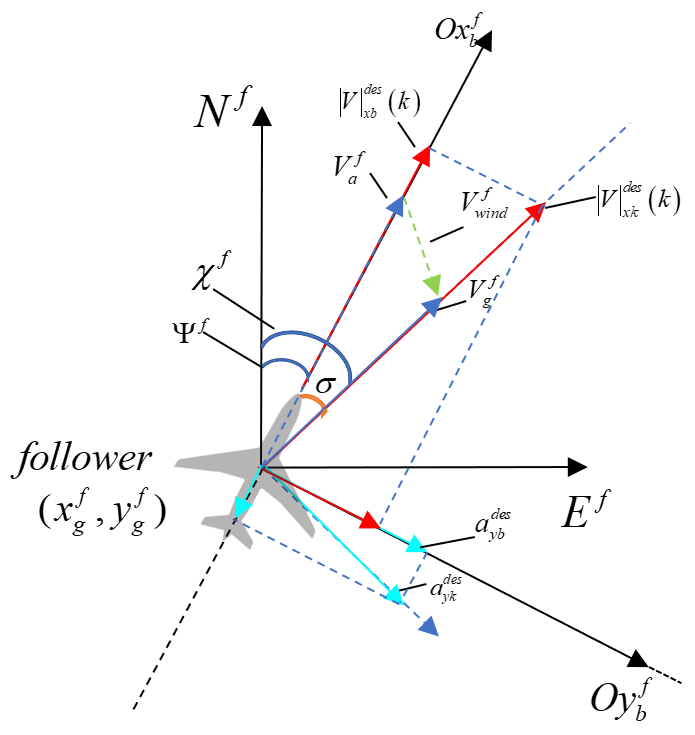
\includegraphics[width=0.5\textwidth]{figures/c3/heavy_wind.png}
    \caption{空速与地速之差较大}\label{fig:heavy_wind}
\end{figure}
图中,风速的大小以及方向已经不能忽略不计,可以得出。原始产生在航迹坐标系$O_kx_ky_kz_k$中的期望速度以及期望与执行机构(油门以及副翼)所在的机体系已有大小为$\sigma$的夹角。
\subsubsection*{风速较大时的改进}
如图\ref{fig:heavy_wind}所示,原始在航迹坐标系之中产生的控制量的期望值若要在机体系之中产生正确的相应,需要进行相应的坐标变换。
\begin{equation}
    \left[
    \begin{matrix}
        control\_input\_x_b(k)\\
        control\_input\_x_y(k)
    \end{matrix}
    \right]
    =  
    \left[  
    \begin{matrix}
        cos\sigma& -sin\sigma\\
        sin\sigma& cos\sigma
    \end{matrix}
    \right]
    \left[
        \begin{matrix}
            |V|_{x_k}^{des}(k)\\
            a_{y_k}^{des}(k)
        \end{matrix}
        \right]
\end{equation}
但是由于机体系两个通道所能够接受的的控制量并不是一致的,需要进行工程化处理:
\begin{equation}
    \left\{
        \begin{aligned}
            &control\_input\_x_b(k)=cos\sigma|V|_{x_k}^{des}(k)+\sum_{n=1}^k\{-sin[\sigma(n)]a_{y_k}^{des}(n)T\}\\
            &control\_input\_x_y(k)=\frac{1}{T}\{sin[\sigma(k)|V|_{x_k}^{des}(k)]-sin[\sigma(k-1)|V|_{x_k}^{des}(k-1)]\}+cos\sigma a_{y_k}^{des}(k)
        \end{aligned}
    \right .
\end{equation}
上式中,$T$是控制时间间隔。实际应用时上式中的微分项要考虑低通滤波以及时间间隔问题,积分项应考虑积分饱和问题。
\subsection{无人机飞行性能限幅设计}
考虑到实际系统各个环节的有界性问题,需要按照无人机气动外形尺寸以及基本飞机空气动力学,计算得出的无人机飞行性能参数,作为实际控制时的各个环节物理量的限幅依据。表\ref{tab:takeoff_performance}-\ref{tab:sink_performance}展示了飞机部分飞行性能:
\begin{table}[H]
    \centering
    \caption{无人机起飞、爬升性能} \label{tab:takeoff_performance}
    \begin{tabular*}{0.9\textwidth}{@{\extracolsep{\fill}}c|ccccccc}
    \toprule
        飞行性能&抬轮速度&起飞速度&滑跑距离&起飞时间
        &爬升率&爬升角
        \\
    \midrule
        值&$4.82m/s$&$5.52m/s$&$16.45m$&$7.36s$
        &$5.99m/s$&$31.21°$\\
    \bottomrule
\end{tabular*}
\end{table}
\begin{table}[H]
    \centering
    \caption{无人机平飞性能} \label{tab:task_performance}
    \begin{tabular*}{0.9\textwidth}{@{\extracolsep{\fill}}c|cccc}
    \toprule
        飞行性能&平定常飞空速&最大空速&最小空速&失速迎角%TODO:需要有最大前项加速度
        \\
    \midrule
        值&$11.52m/s$&$43.76m/s$&$4.60m/s$&$9.94°$\\
    \bottomrule
\end{tabular*}
\end{table}
\begin{table}[H]
    \centering
    \caption{无人机机动性能} \label{tab:motive_performance}
    \begin{tabular*}{0.9\textwidth}{@{\extracolsep{\fill}}c|ccccc}
    \toprule
        飞行性能&转弯速率&转弯半径&转弯时间&法向过载系数&最大滚转角%TODO:需要有最大滚转角速度
        \\
    \midrule
        值&$11.56m/s$&$14.31m/s$&$7.80s$&$1.38$&$43.56°$\\
    \bottomrule
\end{tabular*}
\end{table}
\begin{table}[H]
    \centering
    \caption{无人机下降、爬降落性能} \label{tab:sink_performance}
    \begin{tabular*}{0.9\textwidth}{@{\extracolsep{\fill}}c|cccc}
    \toprule
        飞行性能&下降率&下降角&降落速度&滑跑距离
        \\
    \midrule
        值&$10.19m/s$&$60.15m/s$&$5.89m/s$&$14.81m$
        \\
    \bottomrule
\end{tabular*}
\end{table}
\subsection{编队控制器内外环带宽设计}

\subsection{原始数据滤波器设计}
此处所涉及的原始数据,主要是来自领机以及从机的空速计测量的空速信息。此处使用一阶低通滤波器来实现对于空速信息的滤波。下面简单介绍一阶低通滤波器:
一阶低通滤波器又称作一阶惯性滤波器,传递函数形式为标准一阶惯性环节:
\begin{equation}
    V_0=\frac{1}{1+\tau j\omega}
\end{equation}
其中$\tau$是时间常数。转换成时域形式:
\begin{equation}
    V_0=V_i -\tau\frac{dV_0}{dt}
\end{equation}
离散化之后:
\begin{equation}
    V_0(k)=\frac{V_i(k)+\frac{\tau}{T}V_0(k-1)}{1+\frac{\tau}{T}}
\end{equation}
其中,$T$为控制器时间间隔,$T=\frac{1}{f}$。
此种滤波器在使用时需要注意时间常数的选择,时间常数过大,虽然数据波形会相对平滑,但是滞后较为严重。
\chapter{无人机编队整体控制逻辑、仿真环境以及硬件选型}
\label{chap:hardware}
本章主要介绍无人机编队的编队控制算法之外的系统组成部分;之后介绍无人机编队的整体的控制的实现逻辑,之后将介绍无人机编队的动力学仿真环境的搭建。
最后将介绍本次设计之中所用到的无人机型号,自动驾驶仪硬件以及姿态自动驾驶仪内环基本控制逻辑。
\section{无人机编队整体控制逻辑}
本文所设计的编队控制器是以开源自动驾驶仪内环为基础的,自动驾驶仪内环的作用是追踪来自位置环的无人机期望姿态;
算法所运行的软件环境是$ROS(Robot Operating System)$。$ROS$是一个适用于机器人的开源操作系统。它提供了操作系统应有的服务,包括硬件抽象,底层设备控制,常用函数实现,进程间消息传递,以及包管理。它也提供用于获取、编译、编写、和跨计算机运行代码所需的工具和库函数。本次使用的应用程序接口,正是$ROS$下的$mavros$功能包,本功能包的作用是:将来自自动驾驶仪的无人机状态数据由$mavlink$通信协议转换为$ROS$的进程间的通讯的协议;将来自编队控制器的姿态驾驶仪内环的期望姿态角以及期望油门值按照$mavlink$的协议进行编码,从而起到沟通编队控制器以及姿态驾驶仪内环的桥梁作用。软件层面的整体控制逻辑如下图所示:
\begin{figure}[H]
    \centering
    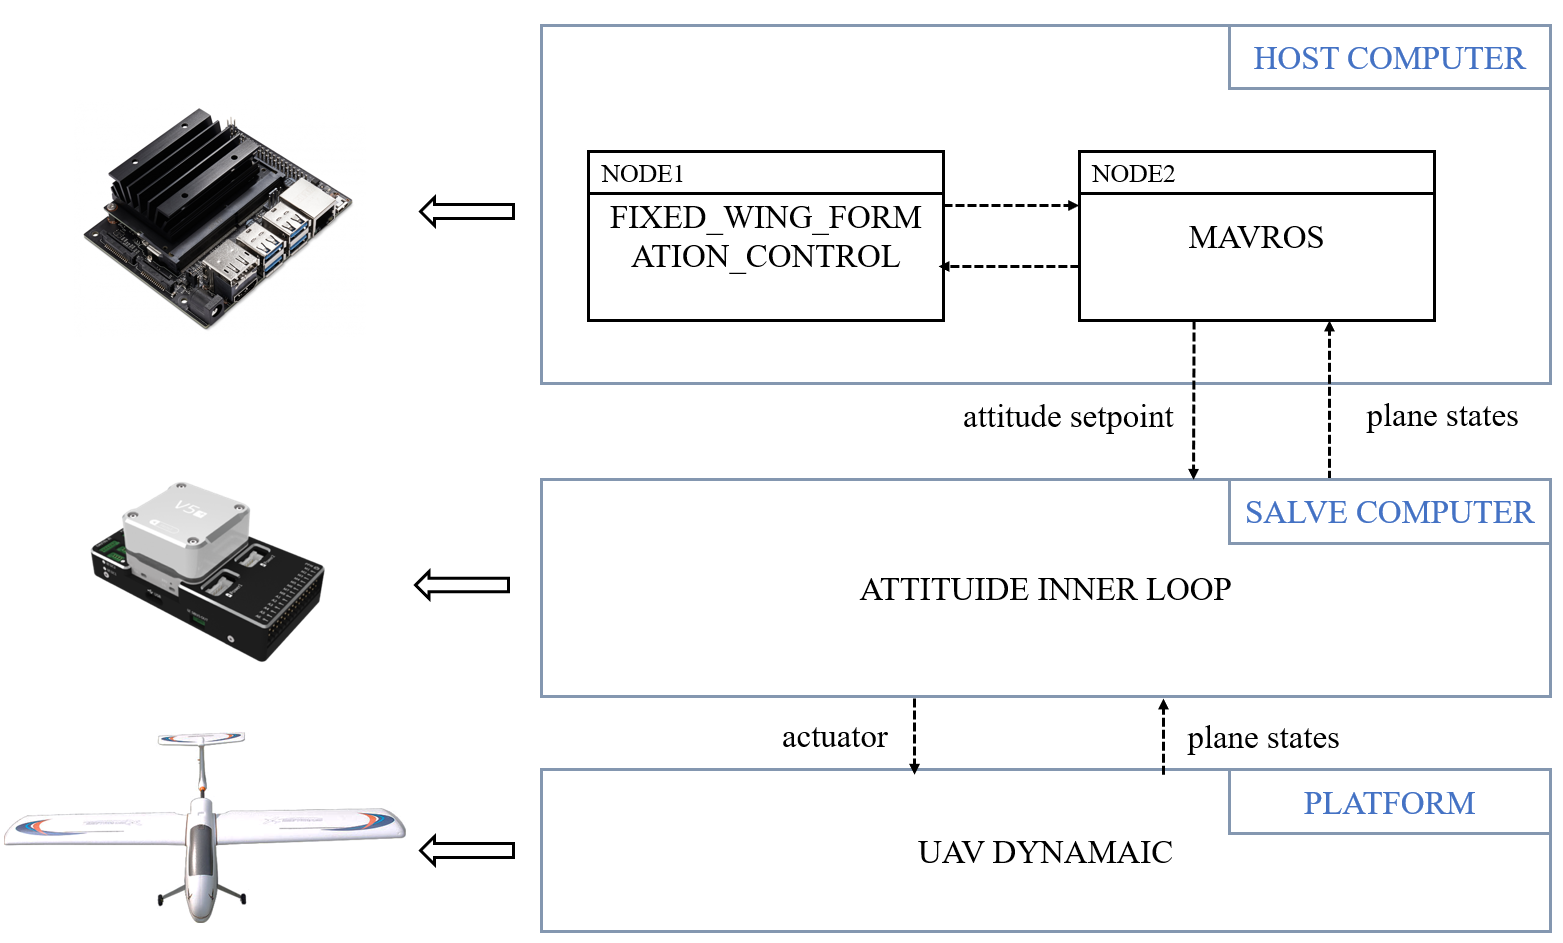
\includegraphics[width=1\textwidth]{figures/c4/c4-soft-hard.png}
    \caption{硬件软件选配关系}\label{fig:c4-soft-hard.png}
\end{figure}

\section{无人机编队仿真环境}
\section{无人机编队硬件选型}
本次毕业设计之中所涉及的编队控制器的自动驾驶仪部分为开源硬件$Pixhawk$:

\chapter{无人机编队整体控制逻辑、仿真环境以及硬件选型}
\label{chap:hardware}
本章主要介绍无人机编队的编队控制算法之外的系统组成部分;之后介绍无人机编队的整体的控制的实现逻辑,之后将介绍无人机编队的动力学仿真环境的搭建。
最后将介绍本次设计之中所用到的无人机型号,自动驾驶仪硬件以及姿态自动驾驶仪内环基本控制逻辑。
\section{ 软件控制逻辑以及软件环境 }
编队控制算法所运行的软件环境是ROS(Robot Operating System)。ROS是一个适用于机器人的开源操作系统。
它提供了操作系统应有的服务,包括硬件抽象,底层设备控制,常用函数实现,进程间消息传递,以及包管理。
它也提供用于获取、编译、编写、和跨计算机运行代码所需的工具和库函数。本次使用的应用程序接口是ROS下的mavros功能包,
本功能包的作用是:将来自自动驾驶仪的无人机状态数据由mavlink通信协议转换为ROS的进程间的通讯的协议;
将来自编队控制器的姿态驾驶仪内环的期望姿态角以及期望油门值按照mavlink的协议进行编码,从而起到沟通编队控制器以及姿态驾驶仪内环的桥梁作用。

自动驾驶仪则使用第\ref{chap:single_control_logic}章中介绍的PX4开源自驾仪,此处不再赘述。
\section{无人机软硬件环境选配}
本文所设计的编队控制器是以开源自动驾驶仪PX4的内环为基础的,PX4的内环自动驾驶仪运行在Pixhawk这一开源硬件之上,成为上层控制的下位机(slave computer):
编队控制算法运行在具有ROS环境的上位机(host computer)中;
整体的软件硬件选配关系如下图所示:
\begin{figure}[H]
    \centering
    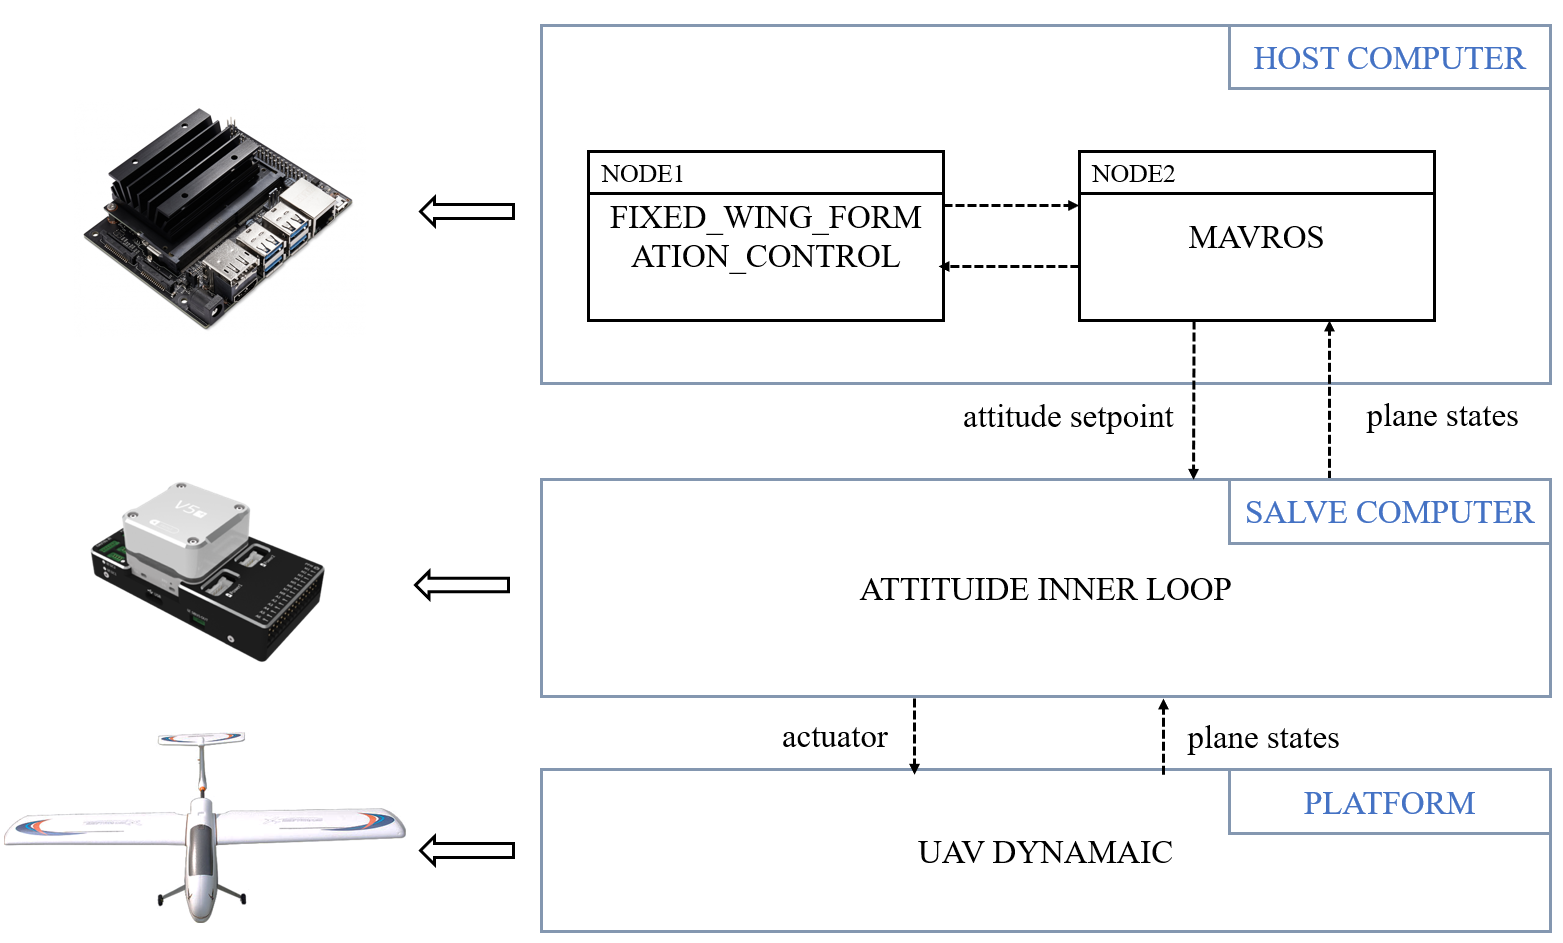
\includegraphics[width=1\textwidth]{figures/c4/c4-soft-hard.png}
    \caption{硬件软件选配关系}\label{fig:c4-soft-hard.png}
\end{figure}
上位机(host computer)的选择主要由其性能决定,应满足ROS基本环境的正常运行以及编队控制算法的需求;其次应考虑该硬件的寿命,体积,工况
要求等指标。下位机(slave computer)是PX4等算法运行的介质,也是飞行之中的重要传感器如惯性原件(IMU)、磁罗盘以及定位模块(GPS Module)的
工作平台,选择时考虑其传感器精度,平台计算能力等因素;无人机是编队控制的载具平台,应根据上述硬件以及必要航电设备选择翼面积、起飞质量
有效载荷等重要参数;根据硬件安放位置选择合适的机舱外形;根据编队控制需要确定平飞速度;根据期望推力选择发动机型号;根据起飞降落方式
选择起落架类型。必要时,应根据性能要求以及指标设计无人机。

在无人机编队过程中,双机通信必不可少。通信模块相对于无人机系统相对独立,在此只介绍硬件实现的一种手段:通讯模块选用P900芯片,通讯协议
选用mavlink协议,驱动由ROS下的串口功能包“serial”提供;实际双机编队飞行试验的硬件链接逻辑如下图所示:
\begin{figure}[H]
    \centering
    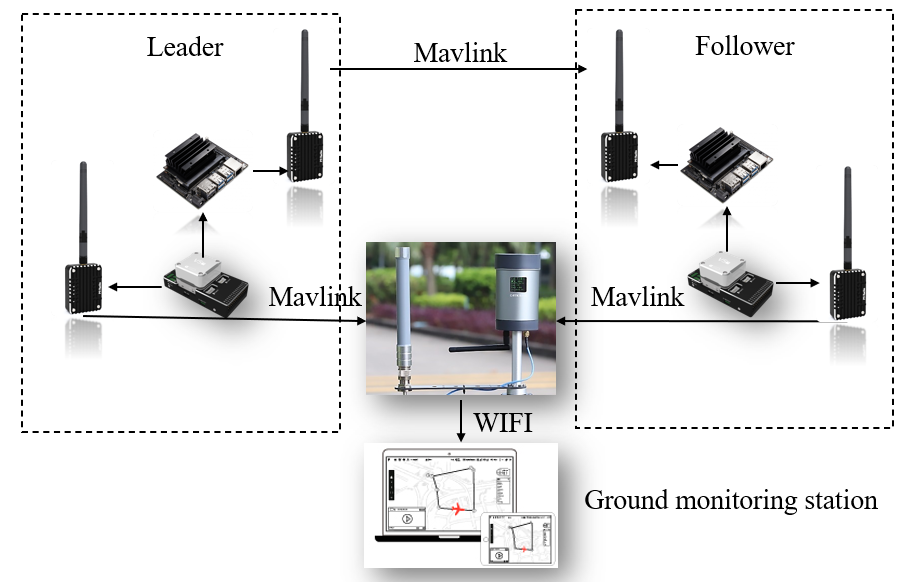
\includegraphics[width=1\textwidth]{figures/c4/double_plane_real}
    \caption{双机编队硬件链接}\label{fig:c4-double_plane_real}
\end{figure}
\section{无人机编队动力学仿真环境}
所谓无人机动力学仿真环境,是在考虑无人机的动力学过程的基础之上搭建的仿真环境,相较于控制器的数学仿真,此种仿真环境考
虑了无人机作为一个实际的被控系统而存在的过渡过程,不确定性以及扰动因素,将更加符合无人机飞行时的实际状态。
本次动力学仿真环境基于Gazebo这一通用的开源仿真环境仿真环境,除调用物理引擎仿真飞行器6自由度的动力学模型外,还可以产生相应的、添加噪声
污染的传感器数据反馈给下位机自动驾驶仪。
\begin{figure}[H]
    \centering
    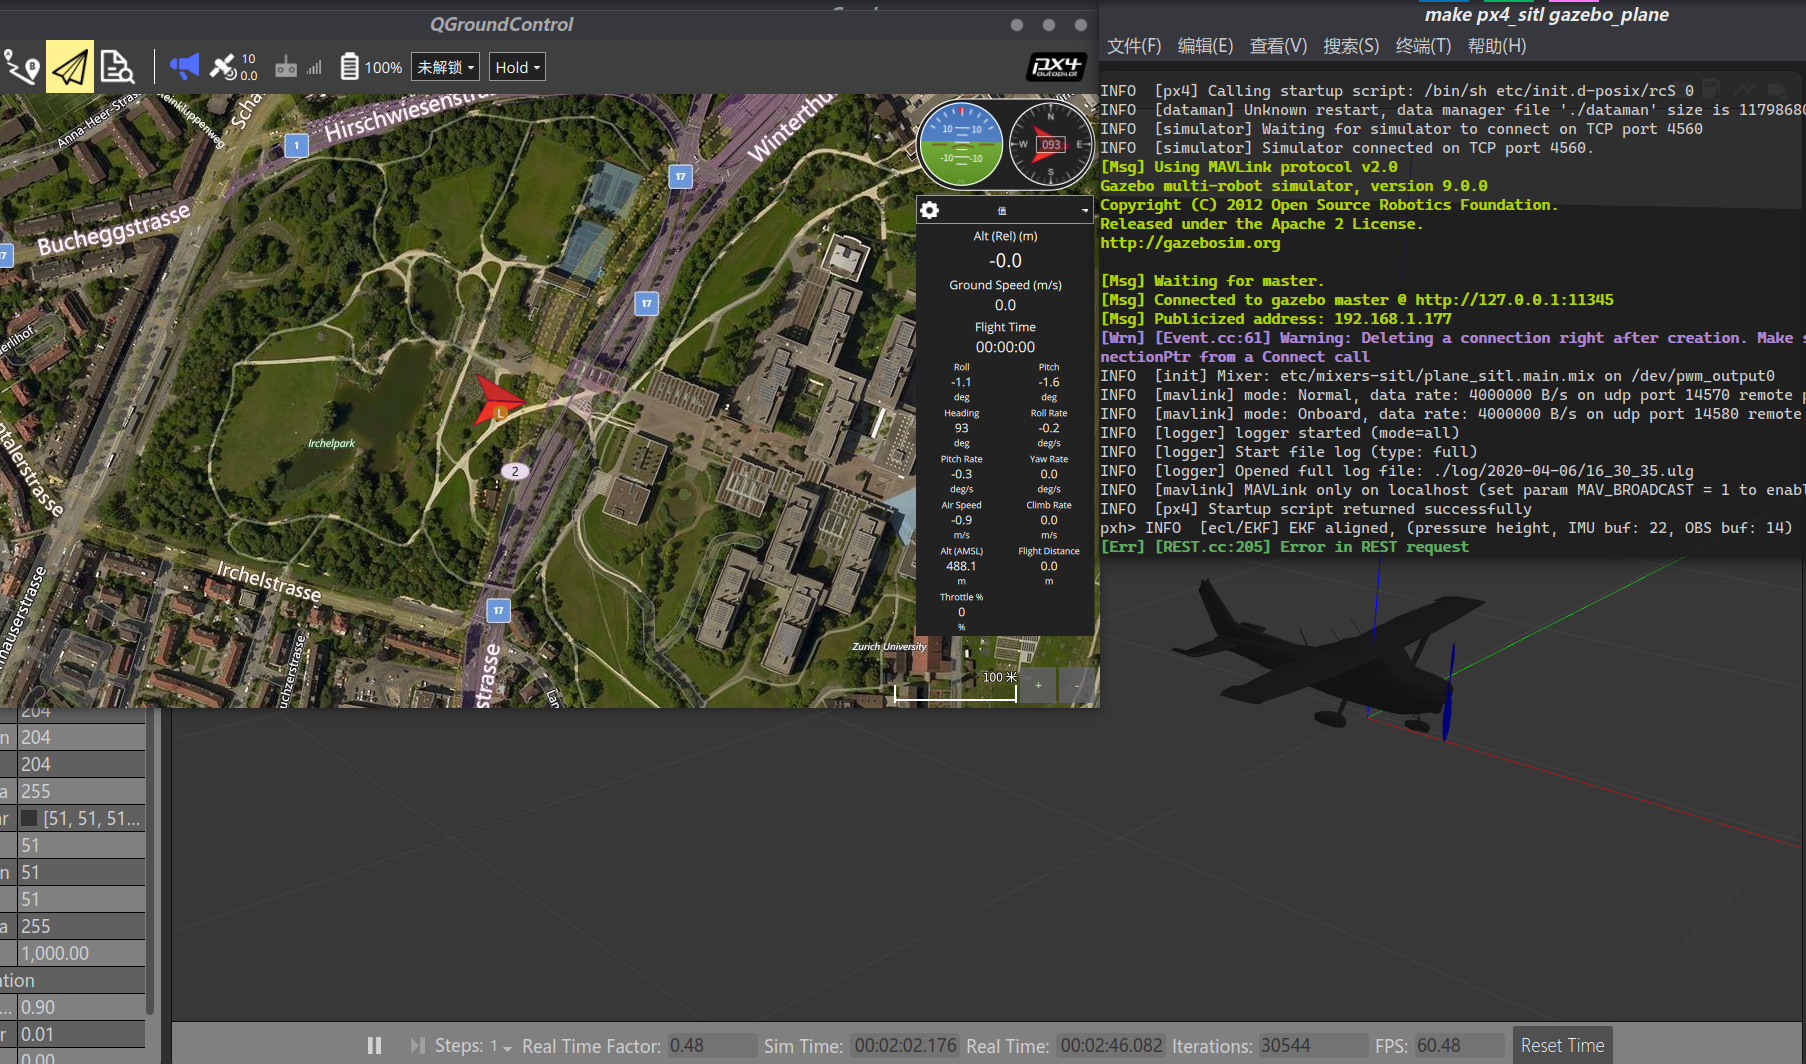
\includegraphics[width=0.75\textwidth]{figures/c4/Gazebo.png}
    \caption{Gazebo仿真环境}\label{fig:c4-Gazebo}
\end{figure}

仿真之中的飞机的动力学模型由Gazebo仿真环境给出,可自定义飞机的质量,推力等参数;仿真之中的传感器数据由Gazebo产生,由PX4读取,作为
真实环境之中的传感器数据的仿真。基于ROS的编队控制程序同时运行,通过mavros等程序API进行数据交互,完成动力学仿真。
相应的仿真程序之间的逻辑关系如下图所示:
\begin{figure}[H]
    \centering
    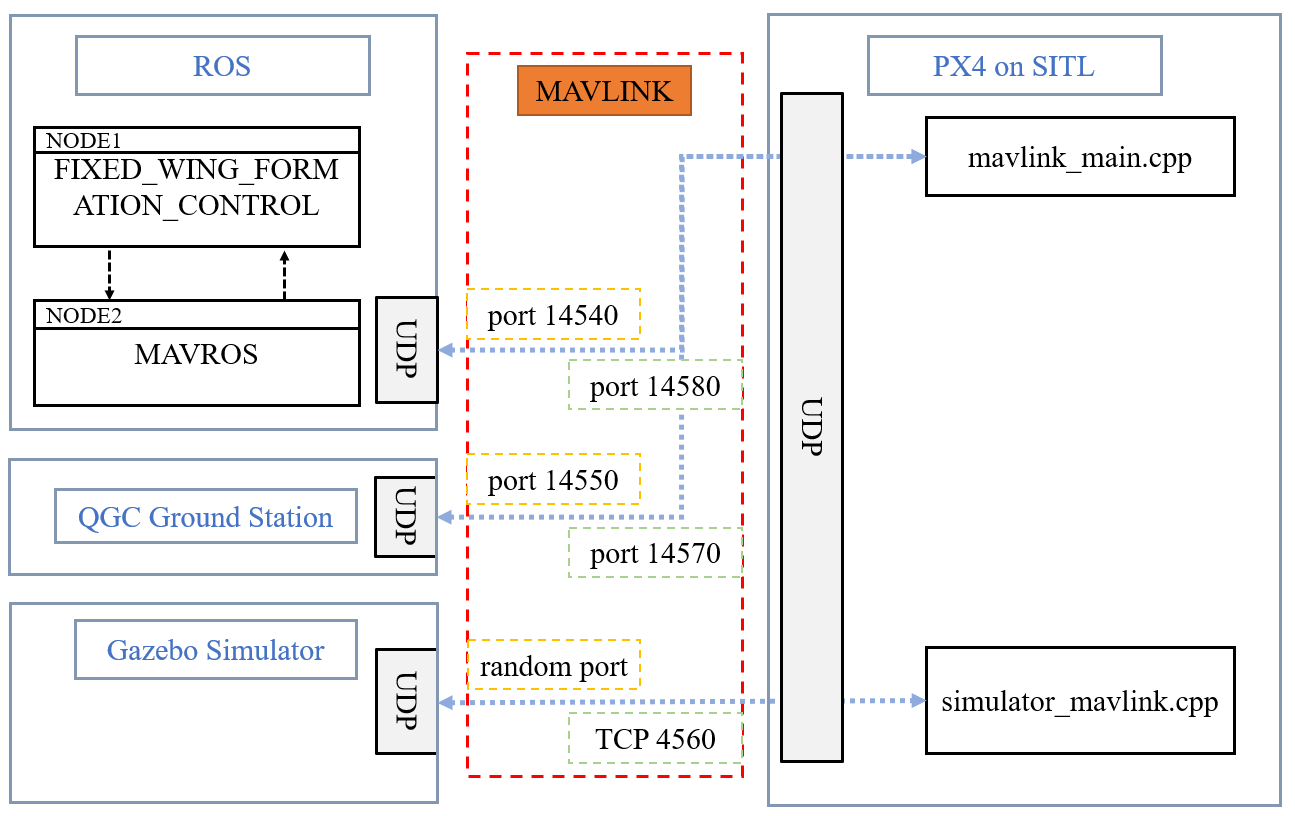
\includegraphics[width=0.75\textwidth]{figures/c4/px4_sitl_overview.png}
    \caption{编队控制仿真逻辑}\label{fig:px4_sitl_overview}
\end{figure}


%%==================================================
%% conclusion.tex for BIT Master Thesis
%% modified by yang yating
%% version: 0.1
%% last update: Dec 25th, 2016
%%==================================================


\begin{conclusion}

本文采用……。{\color{blue}(结论作为学位论文正文的最后部分单独排写,但不加章号。结论是对整个论文主要结果的总结。在结论中应明确指出本研究的创新点,对其应用前景和社会、经济价值等加以预测和评价,并指出今后进一步在本研究方向进行研究工作的展望与设想。结论部分的撰写应简明扼要,突出创新性。)}

\end{conclusion}

%% 参考文献,五号字,使用 BibTeX,包含参考文献文件.bib

%\bibliography{reference/chap1,reference/chap2} %多个章节的参考文献
\bibliography{reference/chap1}


%%%%%%%%%%%%%%%%%%%%%%%%%%%%%%
%% 后置部分
%%%%%%%%%%%%%%%%%%%%%%%%%%%%%%

%% 附录(章节编号重新计算,使用字母进行编号)
\appendix
\renewcommand\theequation{\Alph{chapter}--\arabic{equation}}  % 附录中编号形式是"A-1"的样子
\renewcommand\thefigure{\Alph{chapter}--\arabic{figure}}
\renewcommand\thetable{\Alph{chapter}--\arabic{table}}

%%==================================================
%% app1.tex for BIT Master Thesis
%% modified by yang yating
%% version: 0.1
%% last update: Dec 25th, 2016
%%==================================================


\chapter{***}

附录相关内容…
 

\chapter{Maxwell Equations}


因为在柱坐标系下,$\overline{\overline\mu}$是对角的,所以Maxwell方程组中电场$\bf
E$的旋度

所以$\bf H$的各个分量可以写为:
\begin{subequations}
  \begin{eqnarray}
    H_r=\frac{1}{\mathbf{i}\omega\mu_r}\frac{1}{r}\frac{\partial
      E_z}{\partial\theta } \\
    H_\theta=-\frac{1}{\mathbf{i}\omega\mu_\theta}\frac{\partial E_z}{\partial r}
  \end{eqnarray}
\end{subequations}
同样地,在柱坐标系下,$\overline{\overline\epsilon}$是对角的,所以Maxwell方程组中磁场$\bf
H$的旋度
\begin{subequations}
  \begin{eqnarray}
    &&\nabla\times{\bf H}=-\mathbf{i}\omega{\bf D}\\
    &&\left[\frac{1}{r}\frac{\partial}{\partial
        r}(rH_\theta)-\frac{1}{r}\frac{\partial
        H_r}{\partial\theta}\right]{\hat{\bf
        z}}=-\mathbf{i}\omega{\overline{\overline\epsilon}}{\bf
      E}=-\mathbf{i}\omega\epsilon_zE_z{\hat{\bf z}} \\
    &&\frac{1}{r}\frac{\partial}{\partial
      r}(rH_\theta)-\frac{1}{r}\frac{\partial
      H_r}{\partial\theta}=-\mathbf{i}\omega\epsilon_zE_z
  \end{eqnarray}
\end{subequations}
由此我们可以得到关于$E_z$的波函数方程:
\begin{eqnarray}
  \frac{1}{\mu_\theta\epsilon_z}\frac{1}{r}\frac{\partial}{\partial r}
  \left(r\frac{\partial E_z}{\partial r}\right)+
  \frac{1}{\mu_r\epsilon_z}\frac{1}{r^2}\frac{\partial^2E_z}{\partial\theta^2}
  +\omega^2 E_z=0
\end{eqnarray}
 

%(其后部分无编号)
\backmatter

% 发表文章目录
%%%==================================================
%% pub.tex for BIT Master Thesis
%% modified by yang yating
%% version: 0.1
%% last update: Dec 25th, 2016
%%==================================================

\begin{publications}{99}

    \item\textsc{高凌}. {交联型与线形水性聚氨酯的形状记忆性能比较}[J].
      化工进展, 2006, 532-535.(核心期刊)
    
\end{publications}

% 致谢
%%==================================================
%% thanks.tex for BIT Master Thesis
%% modified by yang yating
%% version: 0.1
%% last update: Dec 25th, 2016
%%==================================================

\begin{thanks}

本论文的工作是在导师……。

\end{thanks}

% 作者简介(博士论文需要)
%%==================================================
%% resume.tex  for BIT Master Thesis
%% modified by yang yating
%% version: 0.2
%% last update: Feb 16th, 2017
%%==================================================


\begin{resume}

\begin{resumesection}{基本情况}
xxx,男,上海人,1985 年~12 月出生,未婚,
上海交通大学物理系在读博士研究生。
\end{resumesection}

\begin{resumeli}{教育状况}
XXXX 年~9 月至~XXXX 年~7 月,上海交通大学, 本科,专业:XXXX

XXXX 年~9 月至~XXXX 年~7 月,上海交通大学, 硕士研究生,专业:XXXX

XXXX 年~9 月至~XXXX 年~7 月,上海交通大学,
博士研究生(提前攻读博士),专业:XXXX
\end{resumeli}

\begin{resumeli}{工作经历}
无。
\end{resumeli}

\begin{resumeli}{研究兴趣}
XXXXXXX。
\end{resumeli}

\begin{resumeli}{联系方式}
通讯地址:上海市闵行区东川路800号,上海交通大学物理系

邮编:200240

E-mail: abcde@sjtu.edu.cn
\end{resumeli}

\end{resume}



\end{document}
